%!TEX root = fed_truth_finder.tex



\section{Evaluation}

\subsection{Numerical Analysis for Connection Loss}
\label{sec:numeric_analysis}

We have theoretically proven that our algorithm can learn the event confidence and trustworthiness ranking like the original centralized algorithms. This experiment then focuses on how the connection loss would impact FedTruthFinder quantitatively, since the unstable mobile network connection is a key characteristic for mobile crowdsensing. A practical mechanism should be able to fight against the unpredictable connection loss.
In general, participants' connection loss may bring two types of negative impacts to the iterative truth discovery algorithm.


\begin{itemize}
	\item \textbf{A small number of sensed data for truth discovery.} While FedTruthFinder can learn an aggregate truth as long as more than $t$ participants are online, the data sources for the truth would be decreased. This would also affect the performance of the learned truth.
	\item \textbf{Possible failure of the whole algorithm.} If a large number of participants lose the connection and only fewer than $t$ participants remain online, then the whole running process of FedTruthFinder would fail and no result can be learned.
\end{itemize}

Specifically, we conduct the numerical analysis for two parts of FedTruthFinder respectively, i.e., event confidence computation and participant trustworthiness ranking. We vary the probability of one participant losing the connection (denoted as $p_l$). If $p_l=0.01$, a participant has 1\% probability of dropping out of the crowdsensing campaign due to one-time connection loss. Then, if a participant needs to connect to the server for $n$ times, it has $1-(1-p_l)^n$ probability to lose the connection. In the experiment, we test $p_l=0.01/0.05/0.1$ to represent good/moderate/bad connection scenarios.




\subsubsection{Event Confidence Computation}

To compare with FedTruthFinder, we consider the state-of-the-art way to do iterative truth discovery with an SSS-based secure aggregation (SA) protocol \citep{Bonawitz2017PracticalSA,Xu2019EfficientAP}, denoted as \textit{SA}, which can also tolerate a certain level of participant connection loss.
In brief, SA leverages a double-masking method to ensure that the truth discovery can run when some users lose the connection. However, not like FedTruthFinder which only needs a one-time connection for each participant to finish one iteration of $\rho$-computation, SA needs a two-time connection (double-masking).

Figure~\ref{fig:num_sensed_data} shows the number of sensed data for truth discovery in each iteration for FedTruthFinder and SA (the total number of data is set to 100). Literature has shown that the number of iterations for truth discovery is often smaller than 10 \citep{yin2008truth} and thus we set the number of iterations up to 10. FedTruthFinder can always obtain more sensed data than SA as FedTruthFinder needs fewer connections. Especially, when the network connection condition is bad ($p_l=0.1$), the performance improvement of FedTruthFinder over SA is more significant.

Figure~\ref{fig:failure} shows the algorithm failure probability (i.e., fewer than $t$ users are online) for FedTruthFinder and SA (we set the number of participants to 100 and $t$ to 50; we do not plot $p_l=0.01$ as both methods are successful almost all the time). FedTruthFinder can significantly reduce the failure probability compared to SA. For example, when the network connection quality is moderate ($p_l = 0.05$), FedTruthFinder has around $99\%$ probability to finish successfully for 10 iterations; however, SA has only around $1\%$ probability. For the bad connection scenario ($p_l = 0.1$), SA will fail with more than $20\%$ probability from iteration 3, while FedTruthFinder can keep working well until iteration 6. This reveals that, even if both FedTruthFinder and SA cannot finish all the ten iterations due to a bad network connection condition, FedTruthFinder can run a larger number of iterations, making the truth more reliable.


\begin{figure*}[t]%[tbhp]
		\centering
		\begin{subfigure}[$p_l=0.01$]{
			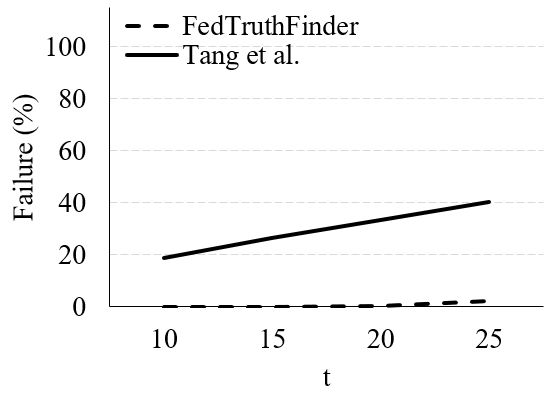
\includegraphics[width=.3\linewidth]{submissions/LeyeWang/fig/fail_trust_0.01.PNG}
			\label{fig:trust_0.01}}
		\end{subfigure}
		\begin{subfigure}[$p_l=0.05$]{
			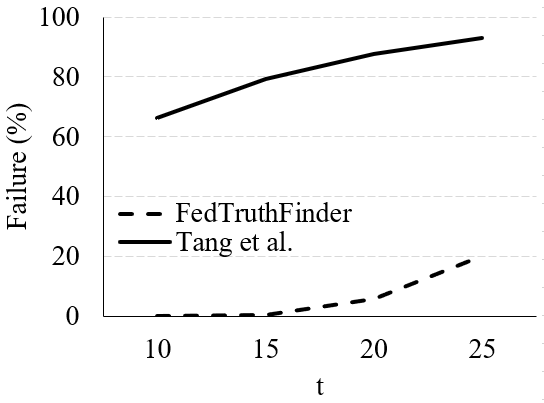
\includegraphics[width=.3\linewidth]{submissions/LeyeWang/fig/fail_trust_0.05.PNG}
			\label{fig:trust_0.05}}
		\end{subfigure}
		\begin{subfigure}[$p_l=0.1$]{
			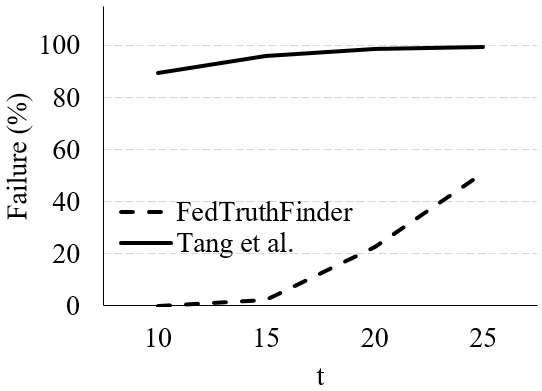
\includegraphics[width=.3\linewidth]{submissions/LeyeWang/fig/fail_trust_0.1.PNG}
			\label{fig:trust_0.1}}
		\end{subfigure}
		\caption{Failure probability of trustworthiness ranking.}
		\label{fig:trust_failure}
\end{figure*}

\begin{figure*}
	\centering
		\begin{subfigure}[Participants number]{
			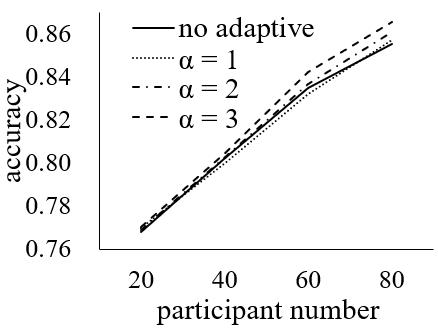
\includegraphics[width=.3\linewidth]{submissions/LeyeWang/fig/truth_acc_traffic_participant_num.PNG}
			\label{fig:acc_vary_participant_num}}
		\end{subfigure}
		\quad
		\begin{subfigure}[Connection loss]{
			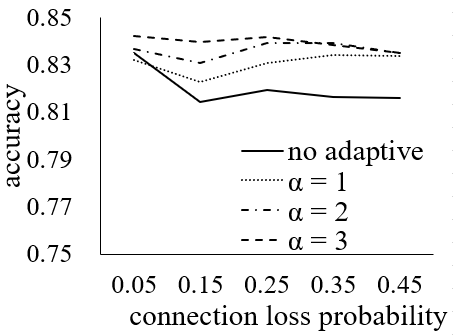
\includegraphics[width=.3\linewidth]{submissions/LeyeWang/fig/truth_acc_traffic_connection_loss.PNG}
			\label{fig:acc_vary_connection_loss}}
		\end{subfigure}
		\caption{Detection accuracy of FedTruthFinder.}
\end{figure*}

\subsubsection{Participant Trustworthiness Rank}

As none of the prior studies have addressed the privacy-preserving trustworthiness ranking problem, we cannot directly find a baseline method to compare. Meanwhile, our proposed trustworthiness ranking algorithm is inspired by the basic idea from \citet{tang2011secure} while significantly enhancing the capability to tolerate participants' connection loss. To this end, we compare FedTruthFinder and \citet{tang2011secure} when certain participants lose connections.

In federated trustworthiness ranking, $t$ is the key parameter related to how many user groups are created, which significantly impacts the algorithm success probability (Theorem 5.3). Suppose the total number of users is 100, we set $t=10/15/20/25$. The algorithm failure probability is shown in Figure~\ref{fig:trust_failure}. With the increase of $t$, the failure probability of FedTruthFinder rises. This fits our expectation as a larger $t$ means that more user groups are generated and the user number per group is reduced. As FedTruthFinder needs at least one user online for each group, smaller user number per group means that the robustness against connection loss is weakened, leading to higher failure probability. Compared to \citet{tang2011secure}, our algorithm significantly increases the success probability when connection is unstable. When $p_l = 0.1$ and $t=10$, the failure probability of our ranking algorithm is 0.04\%, but \citet{tang2011secure} is 96.18\%.
Hence, our algorithm could be an appropriate choice for ranking crowdsensing participants' trustworthiness scores considering the unstable mobile network connection environment.



\subsection{Evaluation of Traffic Light Detection}

We also test FedTruthFinder for traffic light detection, a representative crowdsensing task \citep{ouyang2015truth,wang2013credibility}. We focus on the truth discovery accuracy and the runtime efficiency of FedTruthFinder, which has not been evaluated in the previous numerical analysis.


\begin{figure}[t]
	\centering
	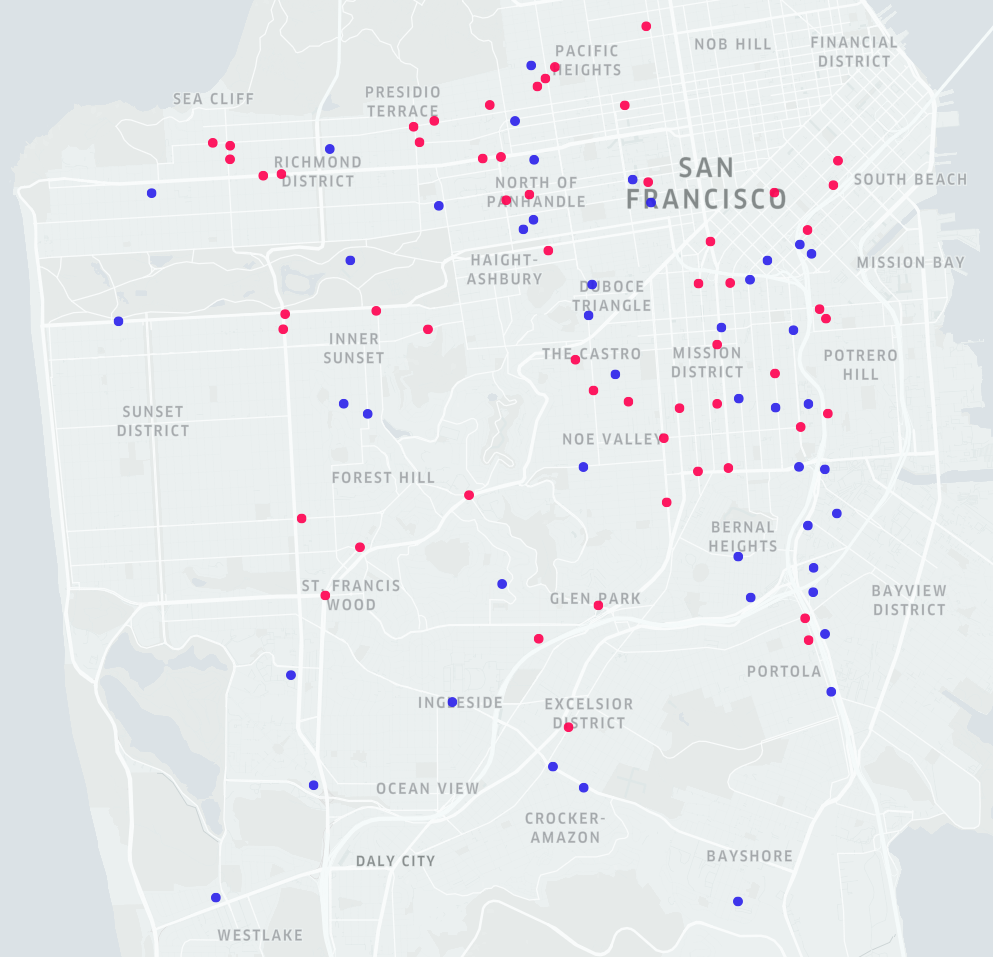
\includegraphics[width=.8\linewidth]{submissions/LeyeWang/fig/traffic_light_map.png}
	\caption{Traffic light event locations (red: true; blue: false). The red points represent the true event locations (i.e, with traffic lights) and the blue points mean the false event locations.}
	\label{fig:traffic_light_map}
\end{figure}

\subsubsection{Data and Tasks} To evaluate FedTruthFinder on the traffic light detection task, we leverage a real-life open dataset including taxis' trajectories. Specifically, the dataset contains time-stamped GPS trajectories from 536 taxis in San Francisco, U.S. in one month of 2008 \citep{epflmobility}. Following \citet{ouyang2015truth}, we manually label 96 traffic light detection event positions using the Street View of Google Maps (Figure~\ref{fig:traffic_light_map}). Then, we randomly select some taxis as participants; their trajectories in the dataset are used to simulate their activities --- if a taxi stops around an event's location, it may report the data. The report error rate (indicating trustworthiness) of each taxi is randomized in $[0,0.5]$. The default participant number is 60 and the connection loss probability is 0.05. The event confidence function is set to `logistic' as it performs better than `sum'. $t$ in SSS is set to half of the total participant number. To increase the randomness, each taxi randomly reports 20\% of the events, and then each setting of the experiment is repeated by 50 times.

\subsubsection{Experiment Platform} Our platform is an Alibaba cloud server with CPU of Intel Xeon Platinum 8163 (12 cores, 2.5GHz) and 24GB memory. The operating system is Ubuntu 20.04. FedTruthFinder is implemented by \textit{Rust} 1.56. \textit{Docker}\footnote{https://www.docker.com/} is adopted to simulate the crowdsensing server and participants.


\subsubsection{Truth Discovery Accuracy} Figure \ref{fig:acc_vary_participant_num} and \ref{fig:acc_vary_connection_loss} plot the accuracy regarding the number of participants and connection loss probability, respectively. Specifically, we compare FedTruthFinder with and without the adaptive truth updating technique (Sec.~\ref{sub:adaptive_truth_updating}). For the adaptive updating, we try $\alpha=1/2/3$ (Eq.~\ref{eq:adaptive_weight}), and find $\alpha=3$ performs the best. The adaptive updating ($\alpha=3$) can consistently improve the accuracy with different participant numbers and connection losses. Specifically, with more participants and higher connection losses, the improvement is more significant. When the connection loss probability increases, the accuracy decreases gradually. This again verifies the effectiveness of FedTruthFinder over SA \citep{Xu2019EfficientAP} --- FedTruthFinder reduces the communication times per truth discover iteration compared to SA, which is conceptually equivalent to the reduction of connection losses in practice.


\begin{figure}[t]%[tbhp]
	\centering
	\begin{subfigure}[Data transmission]{
		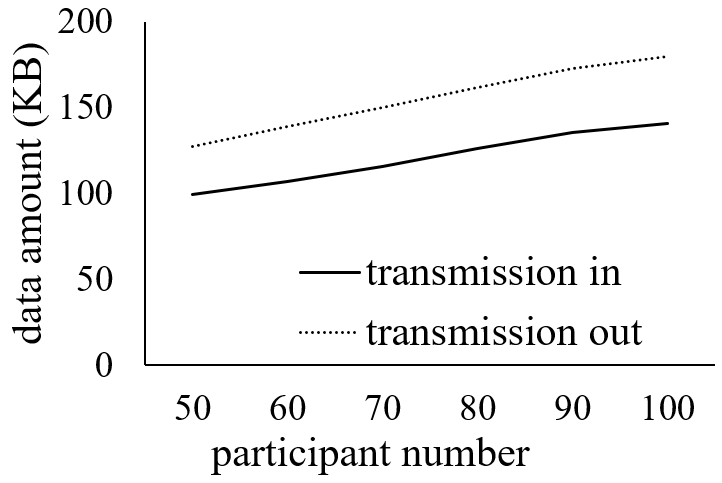
\includegraphics[width=.3\linewidth]{submissions/LeyeWang/fig/data_transmission_traffic.PNG}
		\label{fig:data_transmission}}
	\end{subfigure}
	\
	\begin{subfigure}[Domputation time]{
		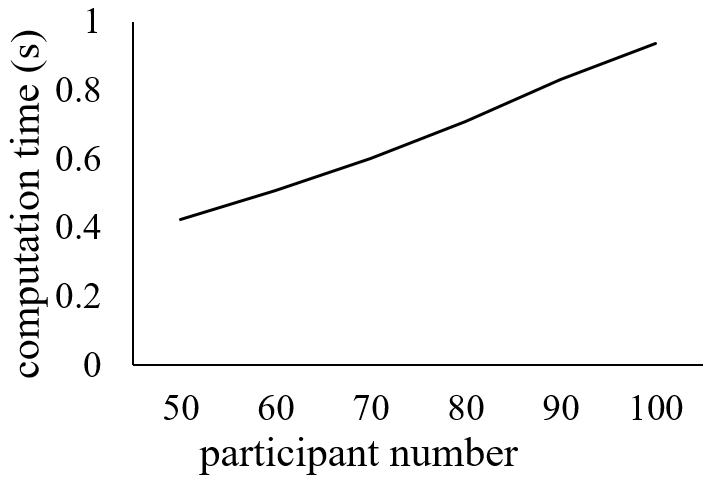
\includegraphics[width=.3\linewidth]{submissions/LeyeWang/fig/computation_time_traffic.PNG}
		\label{fig:computation_time}}
	\end{subfigure}
	\caption{Runtime efficiency of FedTruthFinder.}
\end{figure}

\subsubsection{Runtime Efficiency} Figure~\ref{fig:data_transmission} and \ref{fig:computation_time} record each participant's data transmission amount and computation time, respectively. Note that the computation time is mostly spent in the truth finding step, while the trustworthiness ranking takes only $\sim$0.01s. The results show that the data transmission amount and computation time are both small, verifying the practicality of FedTruthFinder.

